\documentclass{article}
\usepackage{graphicx}
\usepackage{epstopdf}
\usepackage{minx_math}
\usepackage{subfigure,mathtools}

%\usepackage{xypic}
%\xyoption{pdf}

\mathchardef\mh="2D

\begin{document}

\section{3/1/2014}

This note analyzes SCAM where we penalize $\| f \|_\infty$ instead of $\| \partial f \|_\infty$.

\subsection{Changes to Optimization}

The optimization program must change. We modify two formulations of the optimization. The first is the formulation in which we use both $f$ and $\beta$ as variables.

\begin{align*}
\min_{h_k, \beta_k, \gamma_k} & \frac{1}{2n} \sum_{i=1}^n
  \Big( y_i - \sum_{k' \neq k} h_{k' i} - h_{ki} \Big)^2 + \lambda \sum_k \| h_k \|_\infty \\
\textrm{s.t. } & h_{k(i+1)} = h_{k(i)} + \beta_{k(i)}(x_{k(i+1)} - x_{k(i)}) \\
  & \beta_{k(i+1)} \geq \beta_{k(i)}, \mathbf{1} h_k = 0
\end{align*}

Of course, the $\lambda \| h_k \|_\infty$ penalty can be replaced by $\lambda \gamma_k$ and linear inequalities involving $\gamma_k$.\\

Now we reformulate the optimization program that is in term of the discretized second derivative $d_k$.
\begin{align*}
\min_{d_k} &\frac{1}{2n} \| Y - \sum_{k=1}^p \Delta_k d_k \|_2^2 
    + \lambda \sum_{k=1}^p \| \Delta_k d_k \|_\infty \\
\textrm{s.t. } & d_{k(2)}, ..., d_{k(n-1)} \geq 0 \\
& \mathbf{1}_n^\tran \Delta_k d_k = 0 \quad \forall k
\end{align*}

\subsection{Subgradient analysis}

We take the subgradient of the optimization program with $d_k$.

First, we note that the subgradient of the sup-norm $\partial \| x \|_\infty$ at $x=0$ is $\{ z : \sum_i z_i = 1 \}$.

We fix one dimension $k$, let $Y' = Y - \sum_{k' \neq k} \Delta_{k'} d_{k'}$.

The Lagrangian form of the optimization is
\[
\mathcal{L}(d_k, v, \gamma) =
  \frac{1}{2n} \| Y' -  \Delta_k d_k \|_2^2 + \lambda \| \Delta_k d_k \|_\infty
  - \sum_{i=2}^{n-1} v_i d_{ki} + \gamma \mathbf{1}_n^\tran \Delta_k d_k
\]
with the constraint that $v_i \geq 0$ for all $i$. 

We want to find under what conditions does the solution $d_k = 0$ satisfy the KKT conditions.

\[
\partial_{d_k} \mathcal{L} = 
  \frac{1}{n} \Delta_k^\tran ( Y' - \Delta_k d_k) + \lambda \Delta_k^\tran z 
  - v + \gamma \mathbf{1}_n^\tran \Delta_k
\]

where $z \in \partial \| \Delta_k d_k \|_\infty$.

If we evaluate the subgradient at $d_k = 0$, then we have that
\[
\partial_{d_k} \mathcal{L} \Big|_{d_k=0} = \frac{1}{n} \Delta_k^\tran Y' + \lambda \Delta_k^\tran z - v + \gamma \mathbf{1}_n^\tran \Delta_k
\]
where $\| z \|_1 \leq 1$. \\

We want to argue that $d_k = 0$ is an optimal solution. If $d_k = 0$, then complementary slackness and primal feasibility are obvious satisfied. We need only verify stationarity and dual feasibility then.\\

Let us take a brief digression and understand the $\Delta_k$ matrix a little bit more. $\Delta_k$ is $n \times n-1$. Each row corresponds to sample $i$; each column corresponds to an order $(j)$. Each entry $(i,j)$ is $[ X_{ki} - X_{k(j)}]_+$.  Let us reorder the samples so that the $i$-th sample is the $i$-smallest sample. \\

We will construct $\gamma = 0$, and $z = (0, 0, ..., a)$ for some $0 < a < 1$. (coordinates of $z$ correspond to the new sample ordering) We then just need to show that
\begin{align*}
\frac{1}{n} \Delta_k^\tran Y' + \lambda \Delta_k^\tran z &\geq 0 \\
\frac{1}{n} \sum_{i > j} (X_{ki} - X_{kj}) Y'_i + \lambda (X_{kn} - X_{kj})a &\geq 0 \quad 
   \textrm{for each } j \\
\frac{1}{n} \sum_{i > j} \sum_{j < i' \leq i} \mathsf{gap}_{i'} Y'_i 
    + \lambda (X_{kn} - X_{kj})a &\geq 0 \\
\frac{1}{n} \sum_{i' > j} \mathsf{gap}_{i'} \sum_{i \geq i'} Y'_i 
    + \lambda (X_{kn} - X_{kj})a &\geq 0 \\
\frac{1}{n} \sum_{i' > j} \mathsf{gap}_{i'} \mathbf{1}_{i':n}^\tran Y' 
   + \lambda (X_{kn} - X_{kj})a &\geq 0 
\end{align*}

Where $\mathsf{gap}_i = X_{ki} - X_{k,i-1}$. (with respect to ordered indices) The notation $\mathbf{1}_{i':n}$ is a vector that is one on the last $i'$ to $n$ coordinates and zero elsewhere.

Suppose we show that $\frac{1}{n} \mathbf{1}_{i:n}^\tran Y'$ is on the order of $O( \frac{1}{\sqrt{n}})$, then we would be done. Here, we will need to bound $\| Y' \|_\infty$.

$Y'_i = Y_i - \hat{f}(X_i) = f_0(X_i) + w_i - \hat{f}(X_i)$. Both $f_0(X_i)$ and $\hat{f}(X_i)$ are bounded by $2 sLb$. 

For a single $w_i$, we know that with probability at least $1-\delta$, $|w_i| \leq \mathbf{c} \sigma \sqrt{ \log \frac{2}{\delta} }$. Therefore, taking an union bound and setting $\delta = 1/n$, we have that $\max_i |w_i| \leq \mathbf{c} \sigma \sqrt{\log n} $ with probability at least $1 - \frac{1}{n}$. 

Putting this together, $\| Y' \|_\infty \leq \mathbf{c}(sLb + \sigma\sqrt{\log n}) \leq
 \mathbf{c} sLb \sigma\sqrt{\log n}$.\\

Now, we also need to bound the mean of $Y'$: 

\begin{align*}
&\frac{1}{n} \sum_{i=1}^n f_0(X_i) + w_i - \hat{f}(X_i) \\
=& \frac{1}{n} \sum_{i=1}^n f_0(X_i) + w_i 
\end{align*}
The first mean $\frac{1}{n} \sum_{i=1}^n f_0(X_i)$ is the average of $n$ bounded zero-mean random variables since $| f_0(X_i) | \leq 2 s L b$. Therefore, the first term is at most $ sLb \sqrt{\frac{1}{n} \log \frac{2}{\delta}$ with probability at least $1-\delta$.

The second mean is the average of $n$ subgaussian random variables with subgaussian scale $\sigma$. Therefore, the second term is at most $\sigma\sqrt{\frac{1}{n} \log \frac{2}{\delta}}$.

The mean of $Y'$ is therefore at most $\mathbf{c} (sLb + \sigma) \sqrt{ \frac{1}{n} \log n}$ with probability at least $1 - \frac{1}{n}$. 


By Serfling and union bound, with probability at least $1-\frac{1}{n}$, we have that the deviation for all $i$
\begin{align*}
\Big| \frac{1}{n} \mathbf{1}_{i:n}^\tran Y' \Big| &\leq \mathbf{c} sLb\sigma \sqrt{\log n} 
\sqrt{\frac{1}{n} \log 2np} + \mathbf{c} (sLb + \sigma) \sqrt{\frac{1}{n} \log np}\\
  &\leq \mathbf{c} sLb \sigma \sqrt{\frac{1}{n} \log n \log np }
\end{align*}

Plugging this in and plugging in $\lambda > \mathbf{c} sLb \sigma \sqrt{
  \frac{1}{n} \log n \log np}$, we have that:

\begin{align*}
\frac{1}{n} \sum_{i' > j} \mathsf{gap}_{i'} \mathbf{1}_{i':n}^\tran Y' 
   + \lambda (X_{kn} - X_{kj})a &\geq 
 \lambda (X_{kn} - X_{kj}) a 
    - \sum_{i'>j}\mathsf{gap}_{i'} \mathbf{c} sLb\sigma \sqrt{\frac{1}{n} \log n \log np} \\
&\geq \lambda (X_{kn} - X_{kj}) a - (X_{kn} - X_{kj}) 
    \mathbf{c} s Lb \sigma \sqrt{\frac{1}{n} \log n \log np} \\
&\geq 0 
\end{align*}
    

\newpage
\subsection{False Negative Analysis}

Before we begin, we keep in mind that the analysis should be flexible and should be easy to modify to accomodate the following:
\begin{enumerate}
\item choice of norm in the penalty
\item with or without a Lipschitz constraint, boundedness constraint
\end{enumerate}

\subsubsection{Notation}

Where $f : \R^p \rightarrow \R$, we let $\| f \|_P \equiv \E f(X)^2 $.


\subsubsection{Preliminary}
We start with the definitions. Let $y = (y_1, ..., y_n)$ and $y_i = f_0(x_i) + w_i$. We assume $f_0$ to be convex. \footnote{We can probably relax this assumption to be a little bit more general.} We assume that all $x_i \in [-b, b]^s$ \\

\begin{itemize}

\item Let $\mathcal{C}^1$ denote the set of univariate convex functions supported on $[-b,b]$. Let $\mathcal{C}^1_L \equiv \{ f \in \mathcal{C}^1 \,:\, \| \partial f \|_\infty \leq L \}$ denote the set of $L$-Lipschitz univariate convex functions. \\

\item Define $\mathcal{C}^s$ as the set of convex additive functions
\[
\mathcal{C}^s \equiv \{ f \,:\, f = \sum_{k=1}^s f_k, \,
   f_k \in \mathcal{C}^1 \}
\]
\item We will also define classes of bounded and Lipschitz convex additive functions. 
\begin{align*}
\mathcal{C}^s_B &= \{ f \in \mathcal{C}^s \,:\, 
  \| f \|_\infty \leq B \} \\
\mathcal{C}^s_L &= \{ f \in \mathcal{C}^s \,:\, 
f = \sum_{k=1}^s f_k, \, \| \partial f_k \|_\infty \leq L \}
\end{align*}

\item Let $f^*(x) = \sum_{k=1}^s f^*_k(x_k)$ be the population risk minimizer:
\[
f^* = \arg\min_{f \in \mathcal{C}^s} \| f_0 - f^* \|_P^2
\]

\item We let $B$ be an upper bound on $\|f_0\|_\infty$ and $\| f^* \|_\infty$ and let $L$ be an upper bound on $\| \partial_{x_k} f_0 \|_\infty$ and $\| \partial f^*_k \|_\infty$.

\item We define $\hat{f}$ as the empirical risk minimizer:
\[
\hat{f} = \arg\min \{ \| y - f \|_n^2 + \lambda \sum_{k=1}^s \| f_k \|_\infty 
    \,:\, f \in \mathcal{C}^s_L, \mathbf{1}_n^\tran f_k = 0 \}
\]

\item We also define $\hat{f}^*$ as the noiseless empirical risk minimizer:
\[
\hat{f}^* = \arg\min \{ \| f_0 - f \|_n^2 \,:\, 
f \in \mathcal{C}^s_L, \mathbf{1}_n^\tran f_k = 0\}
\]

\item For $k \in \{1,...,s\}$, define $g^*_k$ to be decoupled concave population risk minimizer
\[
g^*_k \equiv \min_{g_k \in \mh \mathcal{C}} \| f_0 - f^*_{-k} - g_k \|_P^2
\]
In our proof, we will analyze $g^*_k$ for $k$'s such that $f^*_k = 0$. 

\item Also, we define the noiseless empirical version:
\[
\hat{g}^*_k \equiv \min_{g_k \in \mh \mathcal{C}_L} \| f_0 - f^*_{-k} - g_k \|_n^2
\]

\item Likewise, we define the empirical version
\[
\hat{g}_k \equiv \min_{g_k \in \mh \mathcal{C}_L} \| y - \hat{f} - g_k \|_n^2
\]
By the definition of the ACDC procedure, $\hat{g}_k$ exist only for $k$ that have zero in their convex additive approximation.

\end{itemize}

\newpage
\subsubsection{Proof outline}


The \textbf{final step} is to show the following:
\begin{align*}
\| f_0 - \hat{f} \|_P & \approx \| f_0 - f^* \|_P \\
\| f_0 - f^* - \hat{g}_k \|_P & \approx \| f_0 - f^* - g^*_k \|_P \quad \trm{for all $k \in \{1,...,s\}$ where $f^*_k = 0$}
\end{align*}
where the difference is a term that decreases with $n$.

Suppose $\hat{f}_k = 0$ and $f^*_k \neq k$, then for large enough $n$, there must be a contradiction because $\| f_0 - f^* \|_P > \| f_0 - f^{*(s-1)} \|_P$. We would have a contradiction.

Suppose $f^*_k = 0$, then $g^*_k \neq 0$. We would have another contradiction.

\rule{5cm}{0.4pt}
\vspace{0.2in}

Concavity, \textbf{removing} sample-dependent convex fucntions.\\

For arbitrary function $g$, we have the following:
\begin{align*}
\| f_0 - \hat{f} - g \|_n = \| f_0 - \hat{f} + f^* - f^* - g \|_n 
   & \leq \| f_0 - f^* -g \|_n
       + \| \hat{f} - f^* \|_n \\
   &\geq \| f_0 - f^* - g \|_n - \| \hat{f} - f^* \|_n 
\end{align*}

Therefore:
\begin{align*}
\| f_0 - f^* - g \|_n^2 - 2 \| f_0 - f^* - g\|_n \| \hat{f} - f^* \|_n \leq
  \| f_0 - \hat{f} - g \|_n^2 \leq
  \| f_0 - f^* -g \|_n^2 + 2 \| f_0 - f^* - g \|_n \| \hat{f} - f^* \|_n 
\end{align*}

The radius of approximation is $2 \| f_0 - f^* - g \|_n \| \hat{f} - f^* \|_n$, which we need to upper bound. $\| f_0 - f^* - g \|_n \leq \mathbf{c} sLb$. 



\rule{5cm}{0.4pt}
\vspace{0.2in}


We \textbf{start} from the definition. We don't need to force $y$ to be zero-mean.

\begin{align*}
\| y - \hat{f} \|_n^2 + \lambda \sum_{k=1}^s \| \hat{f}_k \|_\infty &\leq
  \| y - \hat{f}^* \|_n^2 + \lambda \sum_{k=1}^s \| \hat{f}^*_k \|_\infty \\
\| f_0 + w - \hat{f} \|_n^2 + \lambda \sum_{k=1}^s \Big( \| \hat{f}_k \|_\infty - 
    \| \hat{f}^*_k \|_\infty \Big) &\leq \|f_0 + w - \hat{f}^* \|_n^2 \\
\| f_0 - \hat{f} \|_n^2 + 2\langle w, f_0 - \hat{f} \rangle_n 
     +  \lambda \sum_{k=1}^s \Big( \| \hat{f}_k \|_\infty - 
    \| \hat{f}^*_k \|_\infty \Big) &\leq \| f_0 - \hat{f}^* \|_n^2 + 
    2 \langle w, f_0 - \hat{f}^* \rangle \\
\|f_0 - \hat{f} \|_n^2 - \| f_0 - \hat{f}^* \|_n^2 + 
    \lambda \sum_{k=1}^s \Big( \| \hat{f}_k \|_\infty - 
    \| \hat{f}^*_k \|_\infty \Big) &\leq 2 \langle w, \hat{f} - \hat{f}^* \rangle
\end{align*}

The $\| f_0 - \hat{f} \|_n^2 - \| f_0 - \hat{f}^* \|_n^2$ term is always positive. We want to lower bound the second term with a negative quantity.

One way to proceed:
$\| \hat{f}^*_k \|_\infty \leq 2bL$. And because $\hat{f}^*$ minimizes 

\textbf{Note:}
The $\hat{f}^*$ here could be any function that does depend on the noise. The advantage of having $\hat{f}^*$ is that $\| f_0 - \hat{f} \|_n^2 - \| f_0 - \hat{f}^* \|_n^2 \geq \| \hat{f} - \hat{f}^* \|_n^2$.


\rule{5cm}{0.4pt}
\vspace{0.2in}

\textbf{Continuation from start}.
Taking the \textbf{start} derivation and instead of comparing against $\hat{f}^*$, we will instead compare against $f^*$ (de-meaned).

Since the samples $X_1, ..., X_n$ are clear from context, we denote $\bar{f}^*$ as $\frac{1}{n} \sum_{i=1}^n f^*(X_i)$. 

All parts still work and we get down to the following inequality:
\begin{align*}
\| f_0 - \hat{f} \|_n^2 - \|f_0 - f^* + \bar{f}^* \|_n^2 &\leq 
      2 | \langle w, \hat{f} - f^* + \bar{f}^* \rangle | + \lambda 2sLb \\
  &\leq \mathbf{c} (sLb)^2 \sigma \sqrt{ \frac{1}{n} \log 4n } + 
   \lambda 2 s L b
\end{align*}
with probability at least $1-\frac{1}{n}$.\\


We use the \emph{centering effect} analysis. Since with high probability ($1-\frac{1}{n}$) 
\[
\|f_0 - \hat{f}\|_n^2 - 
  \Big( \|f_0 - f^*\|_n^2 + \mathbf{c} (sLb)^2 \frac{1}{n} \log 4n \Big) \leq 
\|f_0 - \hat{f} \|_n^2 - \|f_0 - f^* + \bar{f}^*\|_n^2
\]
Therefore, with probability at least $1-\frac{2}{n}$,
\begin{align*}
\|f_0 - \hat{f}\|_n^2 - \|f_0 -f^*\|_n^2 &\leq \mathbf{c}(sLb)^2 \frac{1}{n} \log 4n
      + \mathbf{c} (sLb)^2 \sigma \sqrt{\frac{1}{n} \log 4n } + \lambda 2 sLb \\
 &\leq \mathbf{c} (Lb)^2\sigma \sqrt{\frac{s^4}{n} \log 4n} + \lambda 2 sLb
\end{align*}


Now, we use the the \emph{uniform convergence} result. With probability at least $1-\frac{3}{n}$

\begin{align*}
\| f_0 - \hat{f}\|_P^2 - \| f_0 - f^*\|_P^2 & \leq
   \mathbf{c} (Lb)^2 \sigma \sqrt{\frac{s^4}{n} \log 4n} + \lambda 2 s Lb +
   \mathbf{c} (Lb)^3 \sqrt{\frac{s^5}{n^{4/5}} \log 2n} \\
 &\leq \mathbf{c} (Lb)^3 \sigma \sqrt{ \frac{s^5}{n^{4/5}} \log 4n} + \lambda 2 s Lb
\end{align*}


\rule{5cm}{0.4pt}
\vspace{0.2in}

\textbf{f convergence}.

Here, our goal is to bound $\| \hat{f} - f^* \|_n^2$.

Since $f^* = \arg\min_{f \in \mathcal{C}^s} \| f_0 - f \|_P^2$, we have that
\begin{align*}
\|f^* - \hat{f} \|_P^2 &\leq \|f_0 - \hat{f} \|_P^2 - \| f_0 - f^* \|_P^2 \\
 &\leq \mathbf{c} (Lb)^3 \sqrt{ \frac{s^5}{n^{4/5}} \log 4n} + \lambda 2s Lb
\end{align*}

Now, by \emph{uniform convergence} again, we have:

\[
\| f^* - \hat{f} \|_n^2 \leq \mathbf{c} (Lb)^3 \sqrt{\frac{s^5}{n^{4/5}} \log 4n} + 
      \mathbf{c} \lambda s L b
\]

\rule{5cm}{0.4pt}
\vspace{0.2in}

\textbf{Centering Effect}

Here, we bound the difference of $\| f_0 - f^* + \bar{f}^* \|_n^2$ and $\| f_0 - f^* \|_n^2$.

\begin{align*}
\| f_0 - f^* + \bar{f}^* \|_n^2 &= \| f_0 - f^* \|_n^2 
    + 2 \langle f_0 - f^*, \bar{f}^* \rangle + \bar{f}^{*2} \\
  &= \| f_0 - f^* \|_n^2 + 2 \bar{f}^* \langle f_0 - f^*, \mathbf{1} \rangle_n + 
    \bar{f}^{*2} \\
  &= \| f_0 - f^* \|_n^2 + 2 \bar{f}^* \bar{f}_0 - \bar{f}^{*2}
\end{align*}


$\bar{f}^* = \frac{1}{n} \sum_{i=1}^n f^*(X_i)$ is the average of $n$ bounded mean-zero random variables and therefore, with probability at least $1-\delta$, $| \bar{f}^* | \leq 4 s L b \sqrt{ \frac{1}{n} \log \frac{2}{\delta} }$.

The same reasoning likewise applies to $\bar{f}_0 = \frac{1}{n} \sum_{i=1}^n f_0(X_i)$.

Taking a union bound and letting $\delta = \frac{1}{n}$, we have that, with probability at least $1- \frac{1}{n}$, 

\begin{align*}
| \bar{f}^* | | \bar{f}_0 | &\leq \mathbf{c} (sLb)^2 \frac{1}{n} \log 4 n \\
\bar{f}^{*2} &\leq \mathbf{c} (sLb)^2 \frac{1}{n} \log 4 n
\end{align*}

Therefore, with probability $1-\frac{1}{n}$,
\[
\|f_0 - f^*\|_n^2 - \mathbf{c} (sLb)^2 \frac{1}{n} \log 4 n \leq
    \| f_0 - f^* + \bar{f}^* \|_n^2 \leq 
\|f_0 - f^*\|_n^2 + \mathbf{c} (sLb)^2 \frac{1}{n} \log 4 n
\]

\rule{5cm}{0.4pt}
\vspace{0.2in}

\textbf{Denoising}

Here we outline how to bound $\langle w, \hat{f} - \hat{f}^* \rangle$ where $\hat{f}^*$ can be any function that doesn't depend on $w$.

We suppose that both $\hat{f}, \hat{f}^*s \in \mathcal{C}^s_L$.

By Bronshtein, we know that:
\begin{align*}
\log N_\infty(\epsilon, \mathcal{C}_L^1) &= C bL \epsilon^{-1/2} \\
\log N_\infty(\epsilon, \mathcal{C}_L^s) &= C sbL s^{1/2} \epsilon^{-1/2} 
\end{align*}

Clearly, the covering number would not change if we center the set $\mathcal{C}_L^s$ around $\hat{f}^*$, call this $\mathcal{G}$. The difference $\hat{f} - \hat{f}^* \in \mathcal{G}$

For all $h \in \mathcal{G}$:
\begin{align*}
|\langle w, h \rangle_n | &= |\langle w, h - h_\epsilon \rangle_n | 
     + |\langle w, h_\epsilon \rangle_n | \\
 &\leq \frac{1}{n} \| w \|_1  \epsilon + |\langle w, h_\epsilon \rangle_n \| 
\end{align*}

Therefore
\[
\sup_{g \in \mathcal{G}} | \langle w, h \rangle_n | \leq 
      \frac{1}{n} \|w\|_1 \epsilon + 
      \sup_{h_\epsilon \in \mathcal{G}_\epsilon} | \langle w, h_\epsilon \rangle_n |
\]

The final goal is to show that $\sup_{h \in \mathcal{G}} | \langle w, h \rangle_n | \leq 
\textrm{constants} \cdot \sqrt{\frac{1}{n^{4/5}}}$.


\rule{5cm}{0.4pt}
\vspace{0.2in}

\textbf{Chaining}.

Our goal is to give a precise bound for $\sup_{h \in \mathcal{G}} | \langle w, h \rangle|$.

We first restate the chaining theorem. Suppose $\| g \|_n \leq R$ for all $g \in \mathcal{G}$. 

Suppose $\epsilon > \frac{1}{\sqrt{n}}\sigma \mathbf{c} \int_0^R \sqrt{ \log N_2(t, \mathcal{G}) }dt \vee R $. 
Then we have that
\[
P\Big( \sup_{g \in \mathcal{G}} \langle w, g \rangle_n \geq \epsilon \Big) \leq
  4 \exp \Big( - \frac{ n \epsilon^2}{ \mathbf{c} R^2 \sigma^2} \Big)
\]
In our case, $R \leq sLb$.

Restated, we have that, with probablity at least $1-\delta$,
\[
\sup_{g \in \mathcal{G}} | \langle w, g \rangle_n | \leq 
   \mathbf{c} sLb \sigma \sqrt{ \frac{1}{n} \log \frac{4}{\delta}} + 
      \Big( \int_0^R \sqrt{\log N_2(t, \mathcal{G})}dt \vee R \Big)\, 
       \mathbf{c} \sigma \sqrt{\frac{1}{n}} 
\]

Now we evaluate the integral. Since $N_2(t, \mathcal{G}) \leq N_\infty(t, \mathcal{G})$, we know that $\sqrt{\log N_2(t, \mathcal{G})} \leq \sqrt{C s^{1.5} b L} t^{-1/4}$.

\begin{align*}
\int_0^R \sqrt{\log N_2(t, \mathcal{G})} dt &\leq 
      \sqrt{C s^{1.5} b L} \int_0^R t^{-1/4} dt \\ 
 &= \sqrt{C s^{1.5} b L} \, \frac{4}{3} R^{3/4} \\
 &= \sqrt{C s^{1.5} b L} \, \mathbf{c} (sLb)^{3/4} \\
 &\leq \mathbf{c} (s b L)^2
\end{align*}

Coming back, we have, with probability at least $1-\delta$,
\begin{align*}
\sup_{g \in \mathcal{G}} | \langle w, g \rangle | &\leq 
    \mathbf{c} sLb \sigma \sqrt{ \frac{1}{n} \log \frac{4}{\delta} } + 
    \mathbf{c} (sLb)^2 \sigma \sqrt{ \frac{1}{n} } \\
 &\leq \mathbf{c} (sLb)^2\sigma \sqrt{ \frac{1}{n} \log \frac{4}{\delta} }
\end{align*}

\rule{5cm}{0.4pt}
\vspace{0.2in}

\textbf{Uniform convergence}:

The goal is to bound 
$\sup_{f \in \mathcal{C}^s_L} \Big| \| f_0 - f \|^2_n - \|f_0 - f \|^2_P\Big|$. \\

Again, let $\mathcal{G}$ denote the off-centered set of convex functions, that is, $\mathcal{G} \equiv \mathcal{C}^s_L - f_0$. 

First, note that if $h \in \mathcal{G}$, then $\| h \|_\infty = \| f_0 - f \|_\infty \leq 4 s b L$.

Because $\| h \|_n = \| h - h_\epsilon + h_\epsilon \|_n$, we have that
\begin{align*}
\|h_\epsilon \|_n - \| h - h_\epsilon \|_n &\leq 
    \| h \|_n \leq \|h_\epsilon \|_n + \| h - h_\epsilon \|_n \\
\|h_\epsilon \|_n - \epsilon &\leq 
    \| h \|_n \leq \|h_\epsilon \|_n + \epsilon  \\
\| h_\epsilon \|^2_n - 8 \epsilon (s L b)  &\leq \| h  \|^2_n  \leq
   \| h_\epsilon \|_n^2 + 8 \epsilon (s L b) 
\end{align*}
where we used the fact that $\| h - h_\epsilon \|_n \leq \| h - h_\epsilon \|_\infty \leq \epsilon$ and $ \| h_\epsilon \|_n \leq \| h_\epsilon \|_\infty \leq 4 s L b$.


And likewise:
\begin{align*}
\| h_\epsilon \|^2_P - 8 \epsilon (s L b)  &\leq \| h  \|^2_P \leq
   \| h_\epsilon \|_P^2 + 8 \epsilon (s L b)
\end{align*} 

Therefore, 
\begin{align*}
\sup_{h \in \mathcal{G}}  \Big| \|h\|^2_n - \|h\|^2_P \Big| \leq 
\sup_{h_\epsilon} \Big| \|h_\epsilon\|^2_n - \|h_\epsilon\|^2_P \Big| 
        + \epsilon (16 sLb)
\end{align*}

Since $\| h_\epsilon \|_n^2 = \frac{1}{n} \sum_{i=1}^n h_\epsilon(X_i)^2$ is an average of bounded random variables, we have by Union Bound and Hoeffding Inequality that, with probability at most $1 - \delta$,
\begin{align*}
\sup_{h_\epsilon} \Big| \|h_\epsilon\|^2_n - \|h_\epsilon\|^2_P \Big| &\leq
  (8sLb)^2 \sqrt{ \frac{1}{cn} \big(\log \frac{2}{\delta} 
        + \log N_\infty(\epsilon, \mathcal{C}_L^s) \big) } \\
&\leq (8sLb)^2 \sqrt{ \frac{1}{cn} \big(\log \frac{2}{\delta} 
        + C s^{1.5} Lb \epsilon^{-1/2}   \big) }
\end{align*}

We will set $\epsilon = \frac{1}{n^{2/5}} (C s^{0.5} L b)^2$ and $\delta = \frac{1}{n}$. 
Therefore:
\begin{align*}
\sup_{h_\epsilon} \Big|  \|h_\epsilon\|^2_n - \|h_\epsilon\|^2_P \Big| &\leq
   (8sLb)^2 \sqrt{ \frac{1}{cn} \big(\log \frac{2}{\delta} 
        + s n^{1/5}  \big) } \\
  &\leq (8Lb)^2 \sqrt{ \frac{s^5}{cn^{4/5}} \log 2n }
\end{align*}
And
\begin{align*}
\sup_{h \in \mathcal{G}}  \Big| \|h\|^2_n - \|h\|^2_P \Big| &\leq 
\sup_{h_\epsilon} \Big| \|h_\epsilon\|^2_n - \|h_\epsilon\|^2_P \Big| 
        + \frac{1}{n^{2/5}} C^2 s^2 (Lb)^3 \\
  &\leq (8Lb)^2 \sqrt{ \frac{s^5}{c n^{4/5}} \log 2 n}
     + (CLb)^2 \sqrt{ \frac{s^4}{n^{4/5}} } \\
  &\leq \mathbf{c} (Lb)^3 \sqrt{ \frac{s^5}{n^{4/5}} \log 2n}
\end{align*}


\rule{5cm}{0.4pt}
\vspace{0.2in}

\textbf{Concavity start}.

We start from the very beginning, where $\hat{g}_k$ is defined as $\min_{g_k \in \mathcal{C}^1_L} \| y - \hat{f} - g_k \|_n^2 + \lambda \| g_k \|_\infty$.

\begin{align*}
\| y - \hat{f} - \hat{g}_k \|_n^2 + \lambda \| \hat{g} \|_\infty &\leq
   \| y - \hat{f} - g^*_k \|_n^2 + \lambda \| g^* \|_\infty \\
\| y - \hat{f} - \hat{g}_k \|_n^2 &\leq \| y - \hat{f} - g^*_k \|_n^2 + \lambda 2 Lb \\
 &\\
\| f_0 - \hat{f} - \hat{g}_k + w\|_n^2 & \leq \| f_0 - \hat{f} - g^*_k + w \|_n^2 
   +\lambda 2 Lb \\
\| f_0 - \hat{f} - \hat{g}_k \|_n^2 - \|f_0 -\hat{f} - g^*_k\|_n^2 &\leq
   2 \langle w, \hat{g}_k - g^*_k \rangle_n + \lambda 2Lb
\end{align*}

Using the chaining result, setting $s=1$, we have, with probability at least $1-\delta$,
\begin{align*}
\| f_0 - \hat{f} - \hat{g}_k \|_n^2 - \|f_0 - \hat{f} - g^*_k \|_n^2 &\leq
  \mathbf{c} (Lb)^2 \sigma \sqrt{ \frac{1}{n} \log \frac{4}{\delta} }+ \lambda 2 Lb
\end{align*}

Setting $\delta = 1/n$, using \emph{uniform convergence}, we have
\begin{align*}
\| f_0 - \hat{f} - \hat{g}_k \|_P^2 - \|f_0 - \hat{f} - g^*_k \|_P^2 &\leq
  \mathbf{c} (Lb)^2 \sigma \sqrt{ \frac{1}{n} \log 4n }+ \lambda 2 Lb +
  \mathbf{c} (Lb)^3 \sqrt{\frac{s^5}{n^{4/5}} \log 2n } \\
 &\leq \mathbf{c}(Lb)^3 \sigma \sqrt{\frac{s^5}{n^{4/5}} \log 4n} + \lambda 2 Lb
\end{align*}


\rule{5cm}{0.4pt}
\vspace{0.2in}

Now comes \textbf{concavity removal version 2}.

The goal is to bound radius of approximation between $\| f_0 - \hat{f} - g^*_k \|_P^2$ and $\| f_0 - f^* - g^*_k \|_P^2$ and likewise for $\hat{g}_k$.

\begin{align*}
\| f_0 - \hat{f} - g^*_k \|_P^2 - \| f_0 - f^* - g^*_k\|_P^2 &\leq 
    \| f_0 - \hat{f} \|_P^2 - \|f_0 - f^*\|_P^2 - 2\langle f_0 - \hat{f}, g^*_k \rangle
   + 2 \langle f_0 - f^*, g^*_k \rangle \\
 &\leq \mathbf{c} (Lb)^3 \sqrt{ \frac{s^5}{n^{4/5}} \log 4n} + \lambda 2 sLb + 
    2 | \langle \hat{f} - f^*, g^*_k \rangle |  \\
 &\leq  \mathbf{c} (Lb)^3 \sqrt{ \frac{s^5}{n^{4/5}} \log 4n} + \lambda 2 sLb + 
    2 \| \hat{f} - f^* \|_P \| g^*_k \|_P \\
&\leq  \mathbf{c} (Lb)^3 \sqrt{ \frac{s^5}{n^{4/5}} \log 4n} + \lambda 2 sLb +
   \mathbf{c} 2Lb \sqrt{ (Lb)^3 \sqrt{ \frac{s^5}{n^{4/5}} \log 4n} + \lambda 2sLb} 
\end{align*}

The same bound likewise holds for $\hat{g}_k$.

\rule{5cm}{0.4pt}
\vspace{0.2in}








\newpage
\section{2/15/2014}

The two step procedure for variable selection:

\begin{enumerate}
\item Jointly convex approximation:\\ $\{f^c_k\}_{k=1,..,p} = \arg\min_{f_k \in \mathcal{C}_x} \mathbb{E}\Big( f(X) - \sum_{k=1}^p f_k(X_k) \Big)^2$
\item Separate concave post-processing, for each $k=1,...,p$: \\
$f^v_k = \arg\min_{f_k \in \mathcal{C}_v} 
    \mathbb{E}\Big( f(X) - \sum_{k' \neq k} f^c_{k'}(X_{k'}) - f_k(X_k) \Big)^2$
\end{enumerate}

We consider as irrelevant any $k$ where $f^c_k = 0$ and $f^v_k = 0$.\\

\textbf{Claim:} Let $f : C \rightarrow \R$ where $C = [0,1]^p$. Suppose $p(x)$ is a positive density on $C$ and that it satisfies the boundary-points condition.

Suppose $f(x)$ and $\nabla f(x)$ are continuous and for all $k$, that $\partial_{x_k} p(x \given x_k)$ and $\partial^2_{x_k} p(x \given x_k)$ are also continuous as functions on $C$.


Then, the two step procedure is faithful, that is, $f^c_k = 0$ and $f^v_k =0$ implies that $\partial_{x_k} f(x) = 0$.\\

\begin{proof}
We focus on a specific $k$ and suppose that $f^c_k$ and $f^v_k$ are both $0$.\\

We now invoke proposition~\ref{prop:shape_approx_univariate} by letting $g(x) = f(x) - \sum_{k'\neq k} f^c_{k'}(x_{k'})$. It is easy to verify that derivative continuity requirements on $g$ and $p(x \given x_k)$ are all met. We can therefore conclude that $g^*_k(x) = \E[ f(X) - \sum_{k'\neq k} f^c_{k'}(X_{k'}) \given x_k] = 0$.

We now use corollary~\ref{cor:faithfulness_extension} by letting $\phi(x_{-k}) = \sum_{k'\neq k} f^c_{k'}(x_{k'})$. We therefore derive that $\partial_{x_k} f(x) = 0$ and thus prove faithfulness.

\end{proof}

\subsection{Analysis}

To prove the faithfulness of this procedure, we use the following extension of additive faithfulness.

\begin{corollary} 
\label{cor:faithfulness_extension}
Suppose $p(x)$ is a positive density on $[0,1]^p$ and it satisfies the boundary-points condition.

For any function $\phi(X_{-k})$ that does not depend on $X_k$:
 \begin{align*}
f^*_k(x_k) &= \arg\min_{f_k} \mathbb{E} \Big( f(X) 
           - \phi(X_{-k}) - f_k(X_k) \Big)^2 
      = \mathbb{E}\Big[ f(X) - \phi(X_{-k}) \,|\, x_k\Big] 
\end{align*}
We have that $ f^*_k = 0 \Rightarrow \partial_{x_k} f(x) = 0$.
\end{corollary}

\begin{proof}
Identical to the proof of additive faithfulness.
\end{proof}

We also use the following form of the shape-constrained projection theorem.

\begin{proposition}
\label{prop:shape_approx_univariate}
Let $C \subset \R^p$ be a compact set and let $g : C \rightarrow \R$. Let $p(x)$ be a positive density on $C$ and suppose $\E g(X) = 0$.


Suppose that $\partial_{x_k} g(x)$, $\partial_{x_k} p( x \given x_k)$, and $\partial^2_{x_k} p( x \given x_k )$ are all continuous as functions on $C$. Suppose that $\partial^2_{x_k} g(x) \geq 0$.


Let $f^c_k(x_k) = \arg\min_{f_k \in \mathcal{C}_x} \E \Big( g(X) - f_k(X_k) \Big)^2$ and 
$f^v_k(x_k) = \arg\min_{f_k \in \mathcal{C}_v} \E \Big( g(X) - f_k(X_k) \Big)^2$ be the best convex and concave univariate approximation respectively.

Then, $f^c_k = 0$ and $f^v_k = 0$ iff $g^*_k(x_k) = \E[ g(X) \given x_k ] = 0$.
\end{proposition}

\begin{proof}


First, we will establish that $g^*_k(x_k)$ is twice differentiable and that $\partial^2_{x_k} g^*_k(x_k)$ is lower bounded. 

\begin{align*}
g^*_k(x_k) &= \E[ g(X) \given x_k] \\
  &= \int_{x_{-k}} g(x) p(x \given x_k) \\
\partial^2_{x_k} g^*_k(x_k) &= \int_{x_{-k}} g''(x) p(x \given x_k) +
  2 g'(x) p'(x \given x_k) + g(x) p''(x \given x_k) dx_{-k} 
\end{align*}

The first term $g''(x) p(x \given x_k)$ is strictly positive. By assumption, the remaining terms are continuous and hence bounded on a compact set. $\partial^2_{x_k} g^*_k(x_k)$ is therefore lower bounded.\\

Before proceeding, we also note that because $\E g(X) = 0$, it must be that $\E g^*_k(X_k) = 0$.

Now suppose $f^x_k = 0$ and $f^v_k = 0$. Let $\sigma_k^2$ denote $\E X_k^2$. Then 
\[
\arg\min_{c \in \mathbb{R}} \mathbb{E}\Big( g(X) - c (X_k^2-\sigma_k^2) \Big)^2 = 0
\]
Since optimal $c^* = \frac{\mathbb{E} [ g(X) (X_k^2-\sigma_k^2) ]}{\mathbb{E}[ X_k^2 ]}$, 
we know $\mathbb{E} [ g(X) X_k^2 ] = 
\mathbb{E} \Big[ \mathbb{E}[ g(X) \,|\, X_k] X_k^2 \Big] = 0$.\\

Because $\partial^2_{x_k} g^*_k(x_k)$ is lower bounded, for large enough $\alpha$, $g^*_k(x_k) + \alpha (x_k^2 - \sigma_k^2)$ has a non-negative second derivative and thus is convex. Then
\[
\arg\min_{c \in \mathbb{R}} \mathbb{E}\Big( g(X) 
       - c (g^*_k(X_k) + \alpha (X_k^2 - \sigma_k^2)) \Big)^2 = 0
\]
Again, $c^* = \frac{\mathbb{E}[g(X)\big( 
            g^*_k(X_k) + \alpha (X_k^2 - \sigma_k^2) \big)]}{\mathbb{E}
        \big( g^*_k(X_k) + \alpha (X_k^2 - \sigma_k^2) \big)^2} = 0$, so
\begin{align*}
\mathbb{E}[ g(X) \big( g^*_k(X_k) + \alpha X_k^2 \big) ] &= 
\mathbb{E}[ g(X) g^*_k(X_k) ] \\
& = \mathbb{E}\Big[ \mathbb{E}[g(X) | X_k]  g^*_k(X_k) \Big] \\
& = \mathbb{E} g^*_k(X_k)^2 = 0
\end{align*}
Therefore, $g^*_k(x_k) = 0$.

\end{proof}


\newpage
\section{2/7/2014}

\subsection{Best Shape-Constrained Projection}

Even if a function $f_0$ is non-zero, it may be possible that the best convex approximation is zero. But, it cannot be that the best convex approximation and the best concave approximation are both zero.

\begin{theorem}
Let $f_0: C \rightarrow \R$ be a function with a bounded Hessian; let $p$ be some distribution on $C$.
Suppose 
\[
\argmin_{f \in \mathcal{C}_x \cup \mathcal{C}_v} 
   \E (f_0(x) - f(x))^2  = 0
\]
 then $f_0 = 0$ necessarily.
\end{theorem}

\begin{proof}

Suppose that the $\argmin_{f \in \mathcal{C}_x \cup \mathcal{C}_v} \E( f_0(x) - f(x))^2 = 0$, then it must be that 
\[
\argmin_{c \in \R} \E\Big( f_0(x) - c x^\tran x \Big)^2 = 0
\]
Since the optimal $c$ in the above optimization is 
$c^* = \frac{\E[ f_0(x) x^\tran x ]}{\E (x^\tran x)^2 }$, 
we have that $\E[ f_0(x) x^\tran x]=0$.

We know that there exists a convex function $f'$ such that $f' = f_0 + r x^\tran c$ for some large $r > 0$. 

By assumption and convexity of $f'$, it must be that 
\[
\argmin_{c \in \R} \E\Big( f_0(x) - c f'(x) \Big)^2 = 0
\]
We know by similar argument then that $\E[ f_0(x) f'(x) ] =0$. 

However, $\E[ f_0(x) f'(x) ] = \E[f_0(x)^2 + r f_0(x) x^\tran x ] = \E[ f_0(x)^2]$. This is a contradiction. 

\end{proof}

Thus, if we tried both convex and concave projection and the solution is zero, then we can be sure that the original function is identically zero.

The same argument applies if we consider the best single component approximation:
\[
\argmin_{f_k \in \mathcal{C}_x \cup \mathcal{C}_v} 
\E\Big( f_0(x) - f_k(x_k) \Big)^2
\]
Because $\E[ f_0(x) x_k^2 ] = \E\Big[ \E[f_0(x) \given x_k] x_k^2\Big] 
= \E[ f^*_k(x_k) x_k^2]$.
Thus, we can apply the same argument and use $f^*_k(x_k)$ where needed.

\newpage

\section{1/23/2014}

\subsection{Additive Faithfulness Case Study with Quadratic Function and Gaussian Distribution}

We consider a quadratic function $f(x) = x^\tran H x + c^\tran x$ and a Gaussian distribution $X \sim N(0, \Sigma)$. 

We then have a closed form for the additive approximation.
\begin{itemize}
\item If $f$ does not depend on $x_j$, then $f^*_j(x_j) = 0$.
\item If $f$ depends on $x_j$, then, letting $H_j$ be the $j$-th row of $H$ and $\Sigma_j$ be the $j$-th row of $\Sigma$:
\[
f^*_j(x_j) = H_j^\tran \Sigma_j \frac{1}{\Sigma_{jj}} x_j^2 + c_j x_j
\]

\end{itemize}

Let us assume $\Sigma_{jj} = 1$ for all $j$ and that $c=0$ for convenience. We then have two direct corollaries:

\textbf{Corollary:} We have additive convexity if and only if $\trm{diag}(H \Sigma) \geq 0$.

\textbf{Corollary:} We have additive faithfulness if and only if $\trm{diag}(H \Sigma) \neq 0$.

As an example where additive convexity and additive faithfulness are violated. Let $H = [1, 2; 2, 5]$ and $\Sigma = [1, -c; -c, 1]$. For $c=0.5$, additive faithfulness is violated; for $c > 0.5$, additive convexity is violated.


\begin{proof}
We will show that the $f^*_j(x_j)$'s, so described, satisfy the KKT stationarity equations.
\[
f^*_j(x_j) = \E[ f(x) - \sum_{k \neq j} f^*_k(x_k) \given x_j ]  \qquad \trm{for all } j
\]

To prove this, we use the following conditional mean and conditional covariance property of the multivariate Gaussian distribution.
\begin{align*}
& \E[ x_k \given x_j ] = \Sigma_{jk} \Sigma_{jj}^{-1} x_j \\
& \E[ x_k x_{k'} \given x_j] \trm{ is some constant for all $x_j$ } \\
& \E[ x_k^2 \given x_j ] \trm{ is some constant for all $x_j$ } 
\end{align*}
\end{proof}

Why can Gaussian distribution violate additive faithfulness? Because $\frac{\partial p( x_{-j} \given x_j) }{\partial x_j}$ is always large for some values of $x_{-j}$.

\newpage

\section{1/2/2014}

\subsection{Convex-minus-Quadratic Estimation}

Instead of estimating a convex-plus-concave function, it is theoretically sufficient to estimate a convex-minus-quadratic function. 

\begin{theorem}
Any function $h : \R^d \rightarrow \R$ with a bounded Hessian can be decomposed as $h(x) = f(x) - q(x)$ where $f(x)$ is convex and $q(x)$ is $c x^\tran x$ for some $c \geq 0$. 
\end{theorem}

\begin{proof}
For large enough $c$, the Hessian of $h + c$ is a positive semidefinite. The function $f$ is thus convex.
\end{proof}

Convex-minus-quadratic functions are faster to learn. The optimization program has about twice as few variables. It is also possibly easier to analyze. \\

\subsubsection{Implementation}

For additive modeling, I use the following optimization program. There are two parameters $\lambda$ and $L$. 
\begin{align*}
\min_{f_1, ..., f_p} & \frac{1}{n} \sum_i 
  \Big(y_i - \sum_j f_j(x_{ij}) + c_j x_{ij}^2 \Big)^2 + 
  \lambda \sum_j \| \partial f_j - 2 c_j x_j^2 \|_\infty \\
\trm{s.t. } & f_j \trm{ is convex} \\
  & c_j \geq 0 \quad \trm{ and } \quad c_j \leq L
\end{align*}

The second $L$ parameter is necessary. A similar parameter is required in convex-plus-concave estimation as well, which I will explain in the next section. $L$ can be interpreted as a lower bound on the second derivative of the estimated regression function. We set $L=200$ in experiments.


\textbf{Demonstration:} We estimate a one-dimensional function so that we can visualize the behavior of convex-minus-quadratic functions. We set $lambda = 0$. The result is in figure~\ref{fig:quad}.

Here, $n=300$, the $SNR$ is about $0.6$ (high noise).  \\


\begin{figure}[htp]
\label{fig:quad}
\centering
\includegraphics[scale=0.6]{figs/convex_quad.png}
\end{figure}

\subsection{Tuning Parameters for Convex-plus-Concave Estimation}

Convex-plus-concave estimation is not free of tuning parameters. Arbitrary sum of convex and concave functions can represent any function with a bounded Hessian.\\

In Minhua's original SCCAM implementation, the objective is augmented with a square-penalty on the value of the gradients of $f$ and $g$, the convex and the concave functions. The penalty looks like $10^{-6} \| \trm{gradient} \|_2^2$. This penalty is not just for numerical stability; its magnitude affects the estimation. 

\textbf{Demonstration:}

The experimental set-up is the same as before. The result is in figure~\ref{fig:tuning}

\begin{figure}[htp]
\label{fig:tuning}
\centering
\includegraphics[scale=0.6]{figs/convex_concave_tune.png}
\end{figure}

As one can see, when the tuning parameter (the coefficient for the $\| \trm{gradient} \|_2^2$ penalty) is too small, the estimated function is fitting noise. When the tuning parameter is too large, the estimated function is too smooth.

\subsection{Convex-Concave Separation}

We study the problem of variable selection on a convex-plus-concave function $h$. The approach has two steps: 
\begin{packed_enum}
\item Learn \textbf{sparse non-additive} convex function $f$ and concave function $g$ such that $h = f + g$. This is the separation stage.
\item Apply sparse additive model on $f$ and $g$.
\end{packed_enum}

Preliminary results are favorable. In our experiment, we let $p=30, n=300$. The true function is $h(x) = 2 x_1 x_2$ and uses only the first two variables. The SNR is $4$. $h$ is an example of a function that cannot be consistently estimated by additive modeling.

We can indeed identify the correct variables by applying additive model on $f$ after separation.

\begin{figure}[htp]
\label{fig:after_separation}
\centering
\includegraphics[scale=0.6]{figs/scam_separation.png}
\end{figure}

Without separation however, the additive model indeed fails.


\begin{figure}[htp]
\label{fig:before_separation}
\centering
\includegraphics[scale=0.6]{figs/sccam_before_separation.png}
\end{figure}


\end{document}

\newpage
\section{10/25/2013: Convex + Concave function}

Now we consider variable selection for $h(x) = f(x) + g(x)$ where $f$ is convex and $g$ is concave.

\subsection{Separation Approach}

Here is one line of thought. We are given $h_i = h(x_i)$ for a bunch of sample points. Suppose we can learn the decomposition $f_i + g_i = h_i$, then we can use additive faithfulness to recover the relevant variables of $f$ and $g$.

The separation may not be easy however. Perhaps the following optimization:

\begin{align*}
\min_{\beta, \theta}&\sum_{j=1}^p \Big( \|\beta_j\|_\infty + \| \theta_j\|_\infty \Big) \\
 \trm{s.t. } & h_i = f_i + g_i \\
 & f_i \geq f_{i'} + \theta_{i'}^\tran (x_i - x_{i'}) \\
 & g_i \leq g_{i'} + \beta_{i'}^\tran (x_i - x_{i'}) 
\end{align*}

Of course, we have identifiability issues. There exist two sets of functions $\mathcal{F}$ and $\mathcal{G}$ such that for all $f \in \mathcal{F}$, there exist $g \in \mathcal{g}$ such that $f+g = h$. 

The gradient penalty in the optimization program is then critical because it may let us learn a \textbf{sparse} $f,g$. 

We emphasize that we do not attempt to do variable selection at all in the separation optimization, we only want to recover the values $f_i$ and $g_i$. The sparsity patterns of $\beta$ and $\theta$ are of no importance.


\newpage

\section{(7/26/2013)}

Conditional Likelihood Maximization. We compute the marginalization
$$
p(x) = \int \exp(f(x, \xi)) d \xi
$$
where $x \in \R^{d-1}$.

The overall conditional density is

$\log p(y|x) = \log p(y,x) - \log p(x)$. 



\section{(5/22/2013) Meeting Notes}

The list of concepts that we need to formalize:
\begin{packed_enum}
\item We need a high probability bound on $\|Y\|_2^2$ and therefore on $\| \hat{r} \|_2^2$ as well.
\item We need to impose a hard constraint on derivative of $\hat{f}_s$ for all $s$, and use it to derive a high probability bound on the $l_\infty$ norm of $\hat{r}$.
\item We need to formally argue that $F(X) = \sum_{i=1}^n X_i \hat{r}_i \delta_{ ord(i) > j}$ is a coordinatewise-Lipschitz function
\item We need to formally argue that random sampling of coordinates of $\hat{r}$ converges exponentially to zero.
\item We need to take union bound $np$ times. Each time, we also need to take a union bound between the two terms.
\end{packed_enum}


\section{(5/10/2013) Meeting Notes}

\subsection{Sparsistency}

First, we briefly review our inner approximation short-hand notation:

\[f_k(X_{ki}) = \Delta_k d_k  - c_k \mathbf{1}\]

where $\Delta_k$ is a $n\times n-1$ matrix: $\Delta_{k (ij)} = \left\{ \begin{array}{cc} 0 & \trm{ if } order(i) \leq j \\ X_{ki} - X_{k(j)} & \trm{ else } \end{array} \right.$

$d_k$ is a $(n-1)$-dimensional vector. $d_{k1} = \beta_{k1}$, $d_{ki} = \beta_{ki} - \beta_{k (i-1)}$. Therefore, all coordinates of $d_k$ except the first are positive. 

$c_k$ is a constant to ensure that $\sum_i f_k(X_{ki}) = 0$, that the fitted function is centered.\\

We will, for convenient, use the penalty $h(d_k) = |d_{k1}| + \sum_{i=2}^n d_{k2}$. The penalty that correspond to actual $l_\infty$ norm is $h'(d_k) = \max( |d_{k1}|, d_{k1} + \sum_{i=2}^n d_{k2})$. We claim however that $h'(d_k) \leq h(d_k) \leq 2h'(d_k)$; this is because $h(d_k)$ is at most magnitude of the left-most derivative plus the right-most derivative.

\subsubsection{Proof}

FACT: A bounded convex function on a compact set is Lipschitz. The Lipschitz constant depends on $\max_{x \in C} f(x)$\\

FACT: If $f_k(x_k)$ are $L$-Lipschitz, then $\sum_k f_k(x_k)$ is also $L$-Lipschitz.
\[
| \sum_k f_k(x_k) - \sum_k f_k(x'_k) |^2 \leq \sum_k |f_k(x_k) - f_k(x'_k)|^2 \leq \sum_k L^2| x_k - x'_k |^2 \leq L^2 \| x - x' \|_2^2
\]

FACT: if $X$ is sub-gaussian random vector, then $g(X)$ is also sub-gaussian if $g$ is Lipschitz. This is true by McDiarmid's inequality.\\


Let $\hat{f}_k$ be the optimal solution to the optimization
\[
\frac{1}{2n} \| Y - \sum_{k=1}^p \hat{f}_k(X_k) \|_2^2 + \lambda\sum_{k=1}^p \| \partial \hat{f}_k(X_k)\|_\infty \qquad \hat{f}_k \trm{ convex and } \sum_i \hat{f}_k (x_{ik}) = 0 .
\]
We note that using our reformulation, we can also write our objective as
\[
F(d_1,..., d_p) = \frac{1}{2n} \| Y - \sum_{k=1}^p \Delta_k d_k + c_k \mathbf{1} \|_2^2 + \lambda \sum_{k=1}^p ( |d_{k1}| + d_{k2} ... d_{kn} ) .
\]
We can also write the Lagrangian as 
\[
L(d_1,..., d_p) = \frac{1}{2n} \| Y - \sum_{k=1}^p (\Delta_k d_k + c_k )\|_2^2 + \lambda \sum_{k=1}^p ( |d_{k1}| + d_{k2} ... d_{kn} )  - \sum_{k=1}^p \mu_k^\tran d_k - \sum_{k=1}^p \gamma_k (c_k - \frac{1}{n} \mathbf{1}^\tran \Delta_k d_k)
\]
where for every $k$, $\mu_k$ has to be a positive vector.

\textbf{ASSUMPTIONS: }
\begin{packed_enum}
\item $Y' = f(X_S) + \epsilon$ for some Lipschitz function $f$ and sub-gaussian $\epsilon$. $Y = Y' - \bar{Y'}$.
\item The relevant and irrelevant dimensions $X_S, X_{S^c}$ are independent. (We can relax this into a deterministic irrepresentability condition)
\end{packed_enum}

\textbf{CLAIM:}
If we set $\lambda = O \sqrt{\frac{\log (np) }{ n }}$, then (1) $\hat{f}_{S^c} = 0$ with high probability and (2) $\hat{f}_S$ is the solution to the \emph{restricted} regression $\frac{1}{2n} \| Y - \sum_{s \in S} \hat{f}_s(X_s) \|_2^2 + \lambda\sum_{s \in S} \| \partial \hat{f}_s(X_s)\|_\infty$\\

\textbf{NOTE:} 
\begin{packed_enum}
\item We will assume for now, though I think it can be proven, that $\hat{f}_k$ all have, with high probability, bounded Lipschitz constant independent of $n, p$.
\item We made very weak assumption on the true function $f$ but very strong assumptions on the covariates. I think we can trade-off the two: we can still satisfy the deterministic irrespresentability condition with stronger assumptions on the true $f$ and weaker assumptions on the covariates.
\item The proof is similar to Primal Dual Witness but we take gradient with respect to one dimension at a time. This is much more convenient for our case.
\end{packed_enum}

{\bf PROOF:}
We will show that there exists a sparse solution and that the irrelevant dual variables for this solution has magnitude strictly $< 1$. We will later argue that all solutions must then be sparse also.\\

Define $\hat{f}$ as the solution described in the claim. We will prove stationarity, complementary slackness, on the Lagrangrian.

In particular, we will show that with $\hat{f}$ as constructed, we can set the dual variables to satisfy complementary slackness and stationary conditions: $\nabla_{d_k} L(\hat{d})  = 0$ for all $k$.

Define residue $\hat{r} = Y - \sum_{s \in S} \hat{f}_s(X_s)$. \\

We observe that $\hat{r}$ is independent of $X_{S^c}$ because $\hat{f}_{S}$ is the solution to the restricted regression and is therefore independent of $X_{S^c}$. 

Using the reformulation, we can re-write the Lagrangian $L$, in term of just $f_k$, as the following.
\[
\min_{d_k, c_k}  \frac{1}{2n} \| \hat{r} - \Delta_k d_k + c_k \mathbf{1} \|_2^2 + \lambda \sum_{i=2}^n d_{ki} + \lambda|d_{k1}| - \mu_k^\tran d_k + \gamma_k (c_k - \mathbf{1}^\tran\Delta_k d_k)
\]
First, note that by definition as solution of the restricted regression, for $k \in S$, $\hat{f}_k$ satisfy stationarity with dual variables that satisfy complementary slackness. \\

Now, let us fix $k \in S^c$ and prove that $\hat{d}_k = 0, \hat{c}_k=0$ is an optimal solution. 

\begin{align*}
\partial d_k :& \qquad \frac{1}{n} \Delta_k^\tran ( \hat{r} - \Delta_k \hat{d}_k - \hat{c}_k \mathbf{1}) + \lambda \mathbf{u}_k  - \mu_k - \gamma_k \Delta_k^\tran \mathbf{1} \\
\partial c_k: & \qquad \frac{1}{n} \mathbf{1}^\tran ( \hat{r} - \Delta_k d_k - c_k \mathbf{1}) + \gamma_k
\end{align*}
In the derivatives, $\mathbf{u}$ is a $(n-1)$-vector whose first coordinate is $\partial | d_{k1}|$ and all other coordinates are 1.\\


We now substitute in $\hat{d}_k = 0, \hat{c}_k=0$ and show that the duals can be set in a way to ensure that the derivatives are equal to 0.

\begin{align*}
\frac{1}{n} \Delta_k^\tran\hat{r} + \lambda \mathbf{1}  - \mu_k - \gamma_k \Delta_k^\tran \mathbf{1} &= 0 \\
\frac{1}{n} \mathbf{1}^\tran \hat{r} + \gamma_k & = 0 \\
\end{align*}
Note that $\mathbf{u}$ became $\mathbf{1}$.\\

First, we observe that $\gamma_k = 0$ because $\hat{r}$ has empirical mean 0. All we need to prove then is that 
\[
\lambda \mathbf{1} > \frac{1}{n} \Delta_k^\tran\hat{r}. 
\]
We need strict inequality to later argue that ALL solutions are sparse. We need to prove that $| \frac{1}{n} \Delta_k^\tran\hat{r}|$ is of the order $O\sqrt{ \frac{\log(1/\delta)}{n}}$ with probability at least $1- \delta$. \\

Obvious Facts:
\begin{packed_enum}
\item Column $j$ of $\Delta_k$ is $ \max( X_k - X_{k(j)} \mathbf{1}, 0)$. It is all positive with many zeros for large $j$.
\item Coordinates of $\hat{r}$ are identically distributed but not independent. And $\| \hat{r} \|_2^2 = F_S(\hat{f}_S) \leq F_S(0) = \| Y \|_2^2$. 
\item Columns of $\Delta_k$ and $\hat{r}$ are independent. And $\hat{r}$ sums to 0.
\end{packed_enum}

For $j=1$, the deviation bound is easy. 
\[
\Delta_{k, j}^\tran \hat{r} = (X_k  - X_{k(1)} \mathbf{1})^\tran \hat{r} = X_k^\tran \hat{r} - X_{k(1)} \mathbf{1}^\tran \hat{r} = X_k^\tran \hat{r} 
\]
And because $X_k \in \R^n$ is iid subgaussian vector with mean 0 and is independent of $\hat{r}$, the desired deviation bound holds with the desired probability.\\

Non-obvious Facts:\\
We claim that each coordinate of $\hat{r}$ is at most $O\sqrt{|S| \log(n/\delta)}$ with probability at least $1-\delta$. That is because $\hat{r} = Y - \sum_{k \in S} \hat{f}_k (X_k)$. With probability at least $1-\delta$, for all $i$, $|Y_i | \leq \sqrt{\log(n/\delta)}$. Let us suppose $\hat{f}_S = \sum_{k \in S} \hat{f}_k$ is $L$-Lipschitz, and so 
\[
\max_i | \hat{f}_S(X_S^{(i)})| \leq \max_{i,i'} | \hat{f}_S(X_S^{(i)}) - \hat{f}_S(X_S^{(i')}) | \leq L \max_{i,i'} \| X_S^{(i)} - X_S^{(i')} \| \leq 2L \max_i \| X_S^{(i)} \|
\]



%Now, we recall that $\Delta_k$ and $\hat{r}$ are independent, that $\Delta_k$ is a positive matrix with (whp) bounded entries and that $\hat{r} = r_1 - \bar{r}_1$ where $r_1$ is a $n$-vector of independent zero-mean subgaussian random variables and $\bar{r}_1$ is the empirical mean of $r_1$.

%Every coordinate of $\frac{1}{n} \Delta_k^\tran r_1$ must then be of order $O( \sqrt{\frac{1}{n}})$ by standard concentration and $\frac{1}{n} \Delta_k^\tran \mathbf{1} \bar{r}_1$ must also be of order $O(\sqrt{\frac{1}{n}})$.

%We need to take union bounds across all $n$ coordinates of $\frac{1}{n} \Delta_k^\tran \hat{r}$ as well as all $p-|S|$ irrelevant dimensions. Therefore, setting $\lambda = O \sqrt{\frac{\log (np)}{n}}$ suffices.


\newpage

\section{(5/3/2013) Meeting Notes}

\subsection{Short-hand}

The objective is
\[
\frac{1}{2n} \| Y - \sum_{s=1}^p \hat{f}_s(X_s) \|_2^2 + \sum_{s=1}^p \| \partial \hat{f}_s(X_s)\|_2 \qquad \hat{f}_s \trm{ convex and } \sum_i \hat{f}_s (x_{is}) = 0
\]

Let us try to simplify this form. Let $x_{s(1)} ,..., x_{s(n)}$ be the $n$ samples arranged from small to large.\\

Define $\hat{\beta}_{s1}$ as $\frac{\hat{f}_s(x_{s(2)}) - \hat{f}_s(x_{s(1)})}{x_{s(2)} - x_{s(1)}}$.\\

Then  
\begin{align*}
\hat{f}_s(x_{s(1)}) &= \hat{f}_s(x_{s(1)})  \qquad \trm{ constrained by centering}\\
\hat{f}_s(x_{s(2)}) &= \hat{f}_s(x_{s(1)}) + \hat{\beta}_{s1} (x_{s(2)}-x_{s(1)} )\\
\hat{f}_s(x_{s(t)}) &= \hat{f}_s(x_{s(1)}) + \sum_{t' = 1}^{t-1} \hat{\beta}_{s t'} ( x_{s (t'+1)} - x_{s (t')}) 
\end{align*}

We thus define the notation $\hat{f}_s(x_{si}) = c_s + \hat{\beta}_s^\tran D_{si}$ where $D_{si} \in \R^{n-1}$, and is a vector
\[
D_{si} = [ x_{s(2)} - x_{s(1)}, x_{s(3)} - x_{s(2)}, ..., x_{s(t)} - x_{s(t-1)}, 0, ..., 0] \qquad \trm{ where } t = order(i)
\]

And we have the constraint that $\sum_{i=1}^n \hat{f}_s(x_{si}) = n c_s + \sum_{i=1}^n \hat{\beta}_s^\tran D_{si} = 0$, therefore, $c_s = - \left( \frac{1}{n} \sum_{i=1}^n  D_{si} \right)^\tran \hat{\beta}_s$. 

\textbf{Some additional transformation.} Let's define $\hat{d}_{s(i)}$ as the gradient increment. $\hat{d}_{s(1)} = \hat{\beta}_{s(1)}$, and $\hat{d}_{s(2)} = \hat{\beta}_{s(2)} - \hat{\beta}_{s(1)}$. The convexity constraint translates to the constraint that $\hat{d}_{s(i)} \geq 0$ for all $i > 1$.\\

$\hat{\beta}_{s(i)} = \sum_{j \leq i} \hat{d}_{s(i)}$. 

\[
\hat{f}_s(x_{s(2)}) = \hat{f}_s(x_{s(1)}) + \hat{d}_{s(1)} ( x_{s(2)} - x_{s(1)})
\]

\begin{align*}
\hat{f}_s(x_{s(3)}) &= \hat{f}_s(x_{s(2)}) + \hat{\beta}_{s(2)} ( x_{s(3)} - x_{s(2)}) \\
 &= \hat{f}_s({x_{s(1)}}) + \hat{d}_{s(1)} ( x_{s(2)} - x_{s(1)}) + (\hat{d}_{s(2)}+\hat{d}_{s(1)}) (x_{s(3)} - x_{s(2)}) \\
 &= \hat{f}_s({x_{s(1)}}) + \hat{d}_{s(1)} (x_{s(3)}-x_{s(1)} ) + \hat{d}_{s(2)} (x_{s(3)}-x_{s(2)} )
\end{align*}

\[
\hat{f}_s(x_{s(i)}) = \hat{f}_s({x_{s(1)}}) +\hat{d}_{s(1)} ( x_{s(i)} - x_{s(1)}) + \hat{d}_{s(2)} ( x_{s(i)} - x_{s(2)}) + ... + \hat{d}_{s(i-1)} ( x_{s(i)} - x_{s(i-1)})
\]

Define $\Delta(j, x_{si}) = 0$ if $\trm{order}(i) \leq j$, $x_{si} - x_{s(j)}$ else. The $j$ ranges from $1$ to $n-1$. With this definition, we can re-write

\[
\hat{f}_s(x_{si}) = \hat{d}_{s}^\tran \Delta(x_{si}) \qquad \trm{where $\Delta(x_{si}) \in \R^{n-1}$.}
\]

With the simple constraint that all $\hat{d}_{si} \geq 0$ for $i > 1$.\\

\textbf{Notation:} We will also define $\Delta_s$ as a $(n \times n-1)$ matrix whose $i,j$-th entry is $\Delta(j, x_{si})$. 

With this short-hand, we can write $\hat{f}_s(x_s) = \Delta_s\hat{d}_s$.\\

Row $i$ of $\Delta_s$ is the vector $[ \Delta(1, x_{si}), \Delta(2,x_{si}) ..., \Delta(n-1, x_{si})]$. It is $n-1$ dimensional.\\

Column $j$ of $\Delta_s$ is the vector $[ \Delta(j, x_{s1}), \Delta(j, x_{s2}), ..., \Delta(j, x_{sn}) ]$. \\

\emph{Examples:} $\Delta(j, x_{si}) = \max(x_{si} - x_{s(j)}, 0)$

\subsection{Consistency with Short-hand}

We can now attempt the consistency proof with our short-hand notation.

First, what is the objective? 
\[
\| \partial \hat{f}_s(X_s) \|_\infty = \| \hat{\beta}_{si} \|_\infty 
\]

For simplicity, we can use a different but very similar constraint: $ |\hat{d}_{s0}| + \sum_{i=1}^n \hat{d}_{si}$.

The objective is therefore
\[
\frac{1}{2n} \| Y - \sum_{s=1}^p \Delta_s \hat{d}_s \|_2^2 + \sum_{s=1}^p \left[ |\hat{d}_{s0}| + \sum_{i=1}^n \hat{d}_{si} \right].
\]


\section{(4/19/2013) Meeting Notes}
\subsection{Main Result}

\begin{lemma}
\label{lem:int_reduction}
Let $f(x_1, x_2)$ be a 2D convex function defined on $C = [0,1]^2$. Suppose $h(x_1), g(x_2)$ minimizes $ \int_C | f (x_1, x_2) - h(x_1) - g(x_2) |^2 dx$ among all univariate convex functions.\\

$h(x_1)$ is not a constant function iff $\int_{x_2} f(x_1,x_2) dx_2$ is not constant with respect to $x_1$.
\end{lemma}

This following proposition combined with Lemma~\ref{lem:int_reduction} gives the desired result.

\begin{proposition}
Let $f(x_1, x_2)$ be a bivariate convex function defined on $C = [0,1]^2$. Suppose $f$ is \emph{continuous} on $C$ and is twice differentiable. (It must be continuous on the interior of $C$) \\

The following are equivalent:
\begin{packed_enum}
\item For all $x_2$, $f(\cdot, x_2)$ as univariate functions of $x_1$ are identical.
\item For all $x_2$, the integrals $\int_{x_1} f(x_1, x_2) d x_1$ are identical.
\end{packed_enum}
\end{proposition}

\begin{proof}
The first condition trivially implies the second condition.\\

Suppose that for all $x_2$, the integral $\int_{x_1} f(x_1,x_2) dx_1$ is, without loss of generality, equal to $0$. \\

For a fixed $x_1$, define the \emph{right directional derivative} as 
\[
g(x_1) \equiv \lim_{x_2 \rightarrow 0^+} \frac{f(x_1, x_2) - f(x_1, 0)}{x_2}
\]
This limit has to exist by assumption of continuity and by the fact that $f(x_1, \cdot)$ is a univariate convex function with respect to $x_2$.\\

\textbf{Fact 1:} $\int_{x_1} g(x_1) d x_1 = 0$ because $\int_{x_1} f(x_1, x_2) d x_1 = 0$ for all $x_2$. We can invoke the bounded convergence theorem to make this deduction more formal.\\

\textbf{Fact 2:} Because $f$ is convex, $g(x_1)$ is also a component of the 2-dimensional subgradient $\partial f(x_1,0)$, that is, $g(x_1) = \partial f(x_1, 0)^\tran \mathbf{e}_2$. 

Therefore, for all $x_1$, $f(x_1, x_2) \geq f(x_1, 0) + x_2 g(x_1)$. \\

Since $\int_{x_1} f(x_1, 0) + x_2 g(x_1) dx_1 = 0$ and $\int_{x_1} f(x_1, x_2) dx_1 = 0$, it must be that $f(x_1, x_2) =  f(x_1, 0) + x_2 g(x_1)$ for all $x_1$. \\

The Hessian of $f(x_1, x_2)$ at a point $x_1, x_2$ is of the form
\[
\left[ \begin{array}{cc}
	a & b \\
	b & 0 
	\end{array} \right]
\]
where $a \equiv \partial^2 f(x_1,0)/ \partial^2 x_1$ and $ b \equiv \partial g(x_1) / \partial x_1$.  Note that $a,b$ depend on $x_1$ only. The characteristic polynomial is $-\lambda ( a -\lambda) - b^2$. 

Apply the quadratic formula to solve the characteristic polynomial, we get the solutions $\frac{ a \pm \sqrt{a^2 + 4 b^2}}{2}$. The Hessian is therefore NOT positive-semidefinite unless $b=0$. \\

Thus, $g'(x_1) = 0$ for all $x_1$, and $g(x_1)$ is necessarily $0$.\\
\end{proof}
	
	
\subsection{Lemmas}
\begin{lemma}
Let $f(x)$ be a univariate function, integrable. We approximate $f(x)$ with a constant: $c^* \equiv \min_c \int_C | c - f(x) |^2 dx$.\\
Define $A = \int_C 1 dx$ as the measure of $C$, 
\[
\trm{then we have that} \quad c^* = \frac{1}{A} \int_C f(x) dx
\]
\end{lemma}
\begin{proof} (of lemma)\\

Because the objective is convex with respect to $c$, we can use the KKT theorem. The stationarity condition implies that
\begin{align*}
2 \int_C c^* - f(x) dx &= 0 \\
\int_C c^* dx &= \int_C f(x) dx \\
\end{align*}
\end{proof}

Let us also assume that $C = [0, 1]^2$ for simplicity; $C$ has area 1 and when restricted to either $x_1$ or $x_2$, $C$ is a line with length $1$. \\

We claim that $h(x_1) = \int_ {x_2} f(x_1,x_2) d x_2 - \alpha$ for some constant $\alpha$. Why? If we solve $ \min_h \int_C | f (x_1, x_2) - h(x_1) - g(x_2) |^2 dx$ \emph{without} requiring that $h$ is a convex function, the optimal solution is, by lemma, $ x_1 \mapsto \int_ {x_2} f(x_1,x_2) - g(x_2) d x_2$; but because the sum of convex functions is still convex, the solution actually satisfies the convex requirement; and because $\int_{x_2} g(x_2) d x_2$ is a constant, we can define it to be $\alpha$.\\

Therefore, $h(x_1)$ is a constant function iff for all $x_1$, $\int_{x_2} f(x_1,x_2) dx_2$ is a constant. This proves Lemma~\ref{lem:int_reduction}.\\



A lemma that we might not use.
\begin{lemma}
Let $f$ be a convex function on $C \subset \R^n$. Let $x, y \in C$, then for all $x'$ on the line from $x$ to $y$:
\[
f(x') - f(x) \leq \frac{f(y) - f(x)}{(y-x)} (x' - x)
\]
\end{lemma}

Simply put, if we draw a line, in $R^{n+1}$, from $(x, f(x))$ to $(y, f(y))$, then $f$ applied to $[x,y]$ must lie ``below'' this line.\\

\newpage
\section{(4/12/2013) Meeting Notes}

\subsection{A Summary of Current Affairs}

We have tried fitting piecewise linear convex (PLC) functions, reweighted PLC functions, additive PLC functions, PLC and quadratic functions.\\

Out of all these methods, only reweighted PLC function succeeds in exact variable selection. The reweighted PLC function is however difficult to analyze; we may need to analyze it as we would a ``thresholded'' PLC function.\\

All of these methods however give reasonable results: for reasonably sized $n$, the weights of the irrelevant variables are much smaller than the weights of the relevant variables.\\

This suggest then that we should use a weaker criterion for success, which Minhua has already begun to do.

\begin{definition} (Consistency-like Criterion)\\
Let $f(n,p,s)$ be some scaling function, i.e. $f(n,p,s) = \sqrt{\frac{s\log p}{n}}$.

We declare success if, for some constant $c$ independent of $n,p$:
\begin{align*}
\| \hat{\beta}_j \|_\infty &\geq c \quad \forall j \in S, \; n,p \rightarrow \infty \; f(n,p,s) \rightarrow 0 \\
\| \hat{\beta}_j \|_\infty &\rightarrow 0 \quad \forall j \in S^c
\end{align*}
\end{definition}

I don't know for what scaling function $f(n,p,s)$ does the PLC fitting satisfy the above criterion. Perhaps we can search for an answer via experiments on the cluster.\\

I also suggested a criterion before--stronger than the one I write now--which I think does not hold for PLC methods.
\[
\lim_{n \rightarrow \infty} \frac{\| B_S \|_{1,\infty}}{\|B \|_{1,\infty}} \rightarrow 1
\]

\subsection{A Good Simpler Problem to Consider?}

Multi-task lasso where each task has only one sample:

$p$ dimensions, $k$ tasks. \emph{There is no $n$.}\\

$B$ is $p \times k$. The rows of $B$ are different but have same support.

$Y \in \R^k$. $X$ is $k \times p$.

$ Y  = \trm{diag}(X B) + \epsilon$

\begin{align*}
\min_{B} \frac{1}{2}\| Y - \trm{diag}(XB) \|_2^2 + \lambda \| B \|_{1,\infty}
\end{align*}

\subsection{Reweighted PLC}

\begin{figure}[htp]
\includegraphics[scale=0.8]{../code/figs/reweight_exact2.eps}
\end{figure}

\newpage
\section{(4/5/2013) Meeting Notes}

\subsection{Quadratic Optimization Results}

\begin{align*}
\min_{\mathbf{h}, \mathbf{B}, \mathbf{C},\mathbf{S},\mathbf{D}}
& \frac{1}{2n}\sum_{i=1}^n(y_i - h_i)^2 + \lambda \|C\|_{\infty,1} + \gamma \frac{1}{n} \sum_{ij} S_{ji} \\
\trm{s.t.} & C_B = B, C_D = D, S_{ji} \geq 0 \\
	& S_{ji} = h_j - h_i - B_i^\tran(X^j - X^i) - \sum_{k=1}^p D_{ik} (X^j_k - X^i_k)^2
\end{align*}

\begin{figure}[htp]
\subfigure[$f^*$ is piece-wise linear]{ \includegraphics[scale=0.4]{../code/figs/FigureLin.eps}}
\subfigure[$f^*$ is log-sum-exp]{ \includegraphics[scale=0.4]{../code/figs/FigureLogexp.eps}}
\subfigure[$f^*$ is a sum of quadratic and piece-wise -linear]{ \includegraphics[scale=0.4]{../code/figs/FigureQuadLin.eps}}
\subfigure[$f^*$ is a cubic]{ \includegraphics[scale=0.4]{../code/figs/FigureCube.eps}}
\caption{For all these figures, we have $n=100, p=40, s=3$}
\end{figure}


\begin{figure}[htp]
\subfigure[$n=120, \gamma =0.5$]{ \includegraphics[scale=0.4]{../code/figs/FigureQuadLin.eps}}
\subfigure[$n=120, \gamma =0.05$]{ \includegraphics[scale=0.4]{../code/figs/FigureQuadLin2.eps}}
\subfigure[$n=300,\gamma = 0.5$]{ \includegraphics[scale=0.4]{../code/figs/FigureQuadLin3.eps}}
\caption{For all these figures, $f^*$ is a sum of quadratic and piece-wise linear function.}
\end{figure}

\subsection{Reweighted Plot}

\begin{figure}[htp]
\includegraphics[scale=0.5]{../code/figs/Reweighted_exact_recovery.eps}
\end{figure}

\newpage
\section{(3/28/2013) Meeting Notes}

We know that learning a sparse gradient at one point $x$ is too formidable a task, that is why we impose the $l_\infty-l_1$ penalty to link and sync the learning of all the gradients. 

The $l_\infty-l_1$ penalty seems to not be enough. One idea is to use reweighing. We brainstorm some other ideas in the following note. 

\subsection{K-means and Fused Lasso penalty for Piecewise-Linear Convex Functions}

If the true function is piecewise-linear-convex, then the gradients for many of the $x$'s are the same. Therefore, we can either use the $K$-means formulation or the convex fused lasso penalty $\sum_{i,j = 1,...,n} \| B_i - B_j \|_q$ for some norm.

Preliminary experiments with the $K$-means optimization suggest that this can be effective. We need the true number of ``pieces'' to be small and we need $K$-means to pick up the clusters correctly; the second requirement can be possibly waived if we use the fused lasso penalty.

\begin{figure}
\subfigure[k-means with $K* = 3$]{ \includegraphics{../code/figs/k_means_recovery_K03.eps}}
\subfigure[k-means with $K* = 7$]{ \includegraphics{../code/figs/k_means_recovery_K07.eps}}
\end{figure}

\subsection{Quadratic Term}

If a convex function $f$ is strongly convex at a point $x$, then the linear form is a poor approximation, i.e. $f(y)$ can be much larger than $f(x) + \partial f(x) (y - x)$. The usefulness of the data point $y$ in estimating the gradient at $x$ diminishes as $y$ distances itself from $x$ and the approximation gap widens. \\

A natural method that arises out of this observation is to add an additional quadratic term into the optimization objective:

\begin{align*}
\min_{B, \mathbf{c}} & \frac{1}{n} \sum_{i=1}^n | y_i - h_i|^2 + \| [B; \mathbf{c}] \|_{\infty,1} + S_{ij}  \\
\trm{s.t.} & S_{ij} = h_i - h_j - B_j^\tran (X^i - X^j) - \sum_{k=1}^p \mathbf{c}^j_k (X^i_k - X^j_k)^2 \\
			& S_{ij} \geq 0 \\
			& \mathbf{c}^j \geq 0 \\
\end{align*}

Each $\mathbf{c}^j$ is in $\R^p$ and share the same group penalty as the gradients $B_j$'s.

The optimization is not difficult because the constraints are linear with respect to the new $\mathbf{c}^j$ variables.

\newpage

\section{Some Insight}

Let us again consider this noiseless optimization:
\begin{align*}
& \min_B \| B \|_{\infty, 1}\\
&\trm{s.t. } y_j \geq y_i + B_i^\tran (X^j - X^{i*}) \forall i,j
\end{align*}

First, notice that, because (1) each constraint involves only one $B^i$ and (2) the $y_j$'s are not variables, the optimization can be decomposed into $n$ sub-optimizations each done independently. 

\begin{align*}
& \min_{\beta \in \R^p} \| \beta \|_{1}\\
&\trm{s.t. } y_j \geq y_{i*} + \beta^\tran (X^j - X^{i*}) \forall j
\end{align*}

This optimization is analogous to finding a subgradient at just $X^{i*}$. This decomposition allows us to compare directly with the linear case because now, in both cases, we are solving for a single vector.\\

Let us simply the expression further. Define $\Delta \in \R^{p \times n}$ where the $j$-th row $\Delta_j = X^j - X^{i^*}$, and define $\mathbf{v} \in \R^n$ where $\mathbf{v}_j = y_j - y^{i*}$. Now the optimization takes on a familiar form.

\begin{align*}
& \min_{\beta \in \R^p} \| \beta \|_{1}\\
&\trm{s.t. } \mathbf{v} \geq \beta^\tran \Delta
\end{align*}

The optimization is similar to the linear case, but we have an inequality instead of a strict equality here. The inequality is the culprit!\\

The solution to the optimization will lie on the intersection of the boundary of the constraint set and the boundary of a $L_1$ norm ball of some minimal radius. \\

Let $\hat{\beta}$ be the solution to the above optimization. Because $\hat{\beta}$ lies on the boundary of the constraint set, some inequalities must be equalities. Let $I$ be the set of inequalities which becomes equalities when we plug in $\hat{\beta}$. Then $\hat{\beta}$ is equivalently the solution of the following optimization:

\begin{align*}
& \min_{\beta \in \R^p} \| \beta \|_{1}\\
&\trm{s.t. } \mathbf{v}_I = \beta^\tran \Delta_I
\end{align*}

where $\Delta_I$ is a $p \times |I|$ sub-matrix and $\mathbf{v}$ is a $|I|$-dimensional sub-vector. Now we see the problem: if $|I|$ is very small, then it is as if we are solving lasso with very few samples--$|I|$ number of samples instead of $n$!\\

How do we interpret $I$? Intuitively, I think of it as all $j$ for which $y_j \approx y_{i*} + B_{i*}^\tran (X^j - X^{i*})$. That is, it is the set of points for which the convex function is close to linear. For strongly convex functions like $\|x\|^2_2$, $I$ would be very small. For linear functions like $\beta^{*\tran} x$, $|I| = n$. \\

Therefore, this explains why our optimization gives sparse solution if the true function is linear and highly non-sparse solution if the true function is strongly convex.

\section{Experiments}

In the soft-recovery experiment, we measure $\frac{ \| B_S \|_{\infty,1}}{\|B\|_{\infty, 1}}$.
\begin{figure}
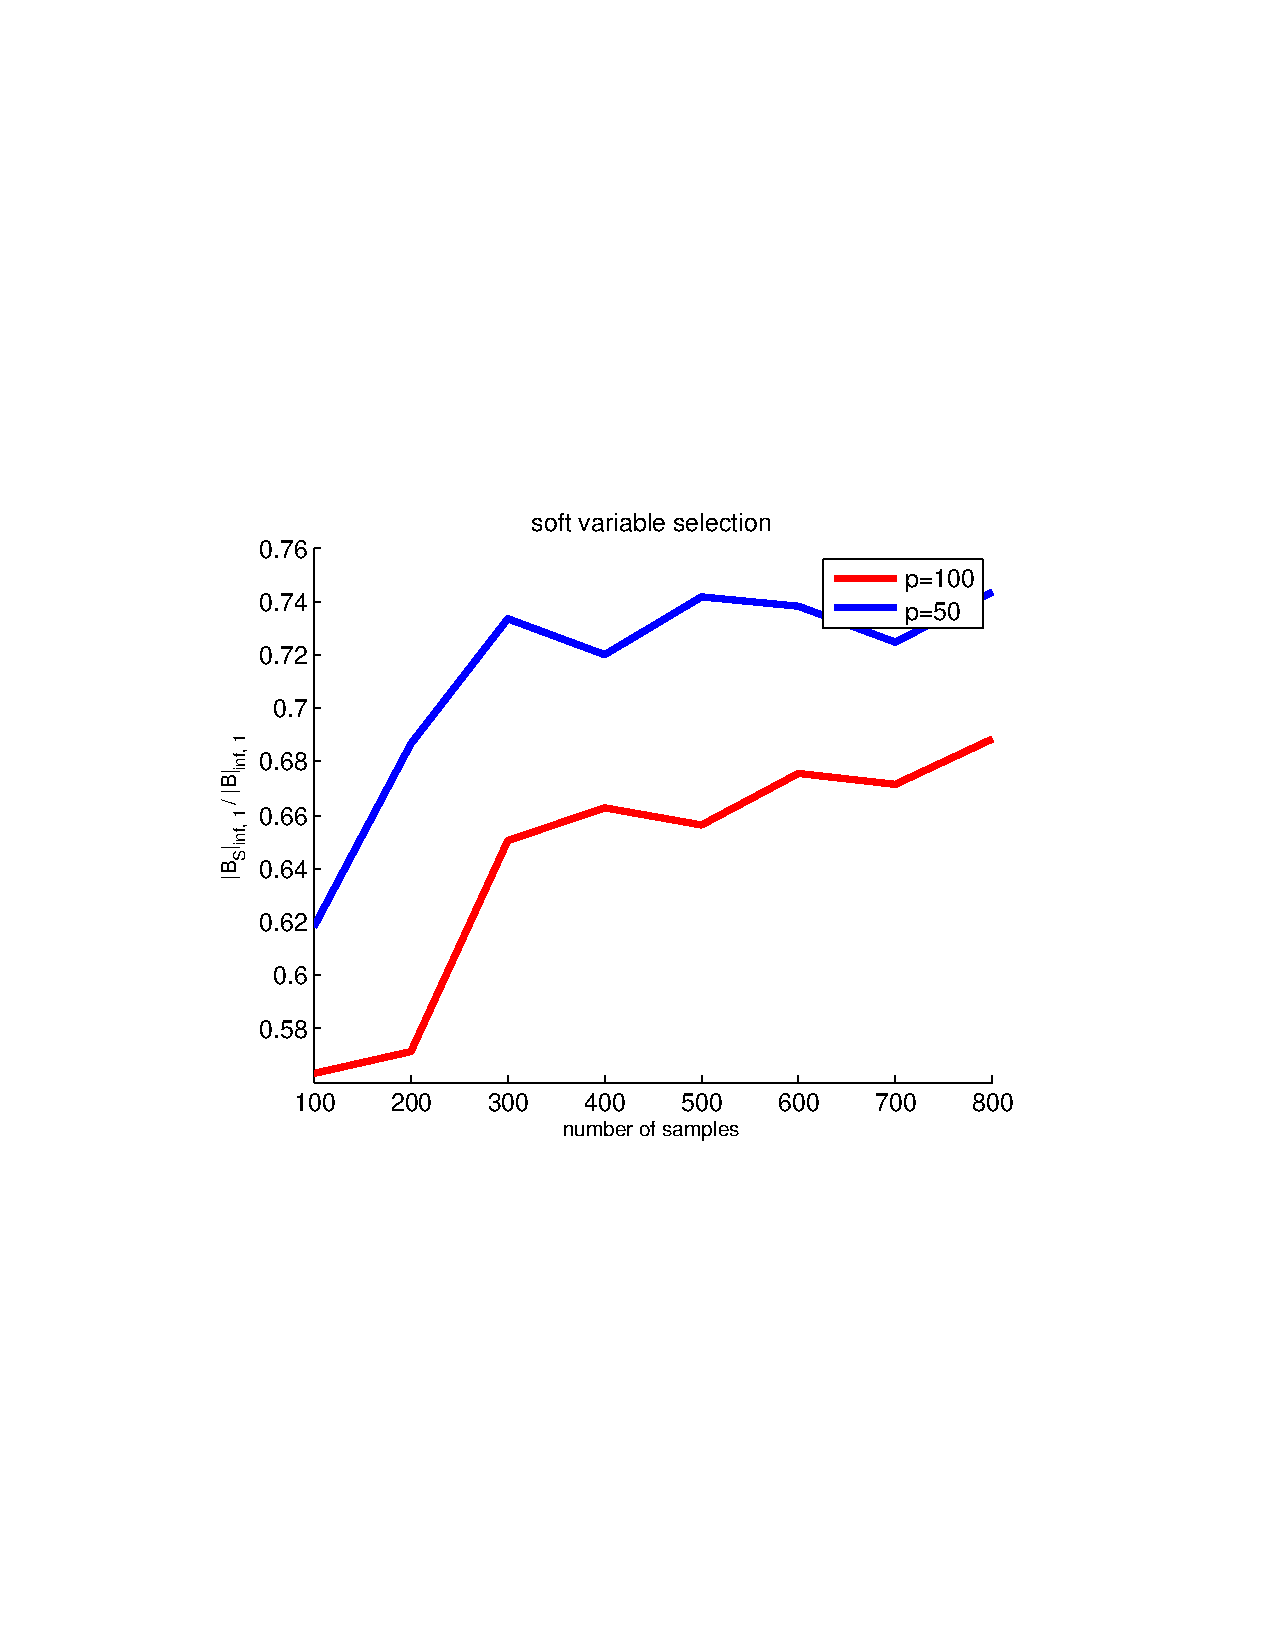
\includegraphics[trim=150 200 150 200]{../code/figs/soft_recovery.pdf}
\end{figure}
The recovery curve plateaus. It should converge to 1 but appears to be doing so very slowly.

As a thought experiment, let's consider a noiseless support recovery optimization:
\begin{align*}
& \min_B \| B \|_{\infty, 1}\\
&\trm{s.t. } y_i \geq y_j + B_j^\tran (X^i - X_j) \forall i,j
\end{align*}
The optimum of this program should become exactly sparse as $n \rightarrow \infty$, but may become sparse at a very slow rate with respect to $n$. The penalized least-square solution then, like a heat-seeking missile thrown off target by a decoy, homes in to the non-sparse optimum rather than the actual sparse solution.

We have not implemented this optimization but can still approximate it with the penalized square error optimization by setting lambda very small.

What we see if that we must weigh the dimensions to exactly recover the support. We must use a weighed form of the objective.

\begin{align*}
& \min_B \sum_{s=1}^p \lambda_s\| B_{s\cdot} \|_{\infty}\\
&\trm{s.t. } y_i \geq y_j + B_j^\tran (X^i - X_j) \forall i,j
\end{align*}

Where $\lambda_s$ is small for $s \in S$ and large for $s \notin S$. 

\begin{figure}
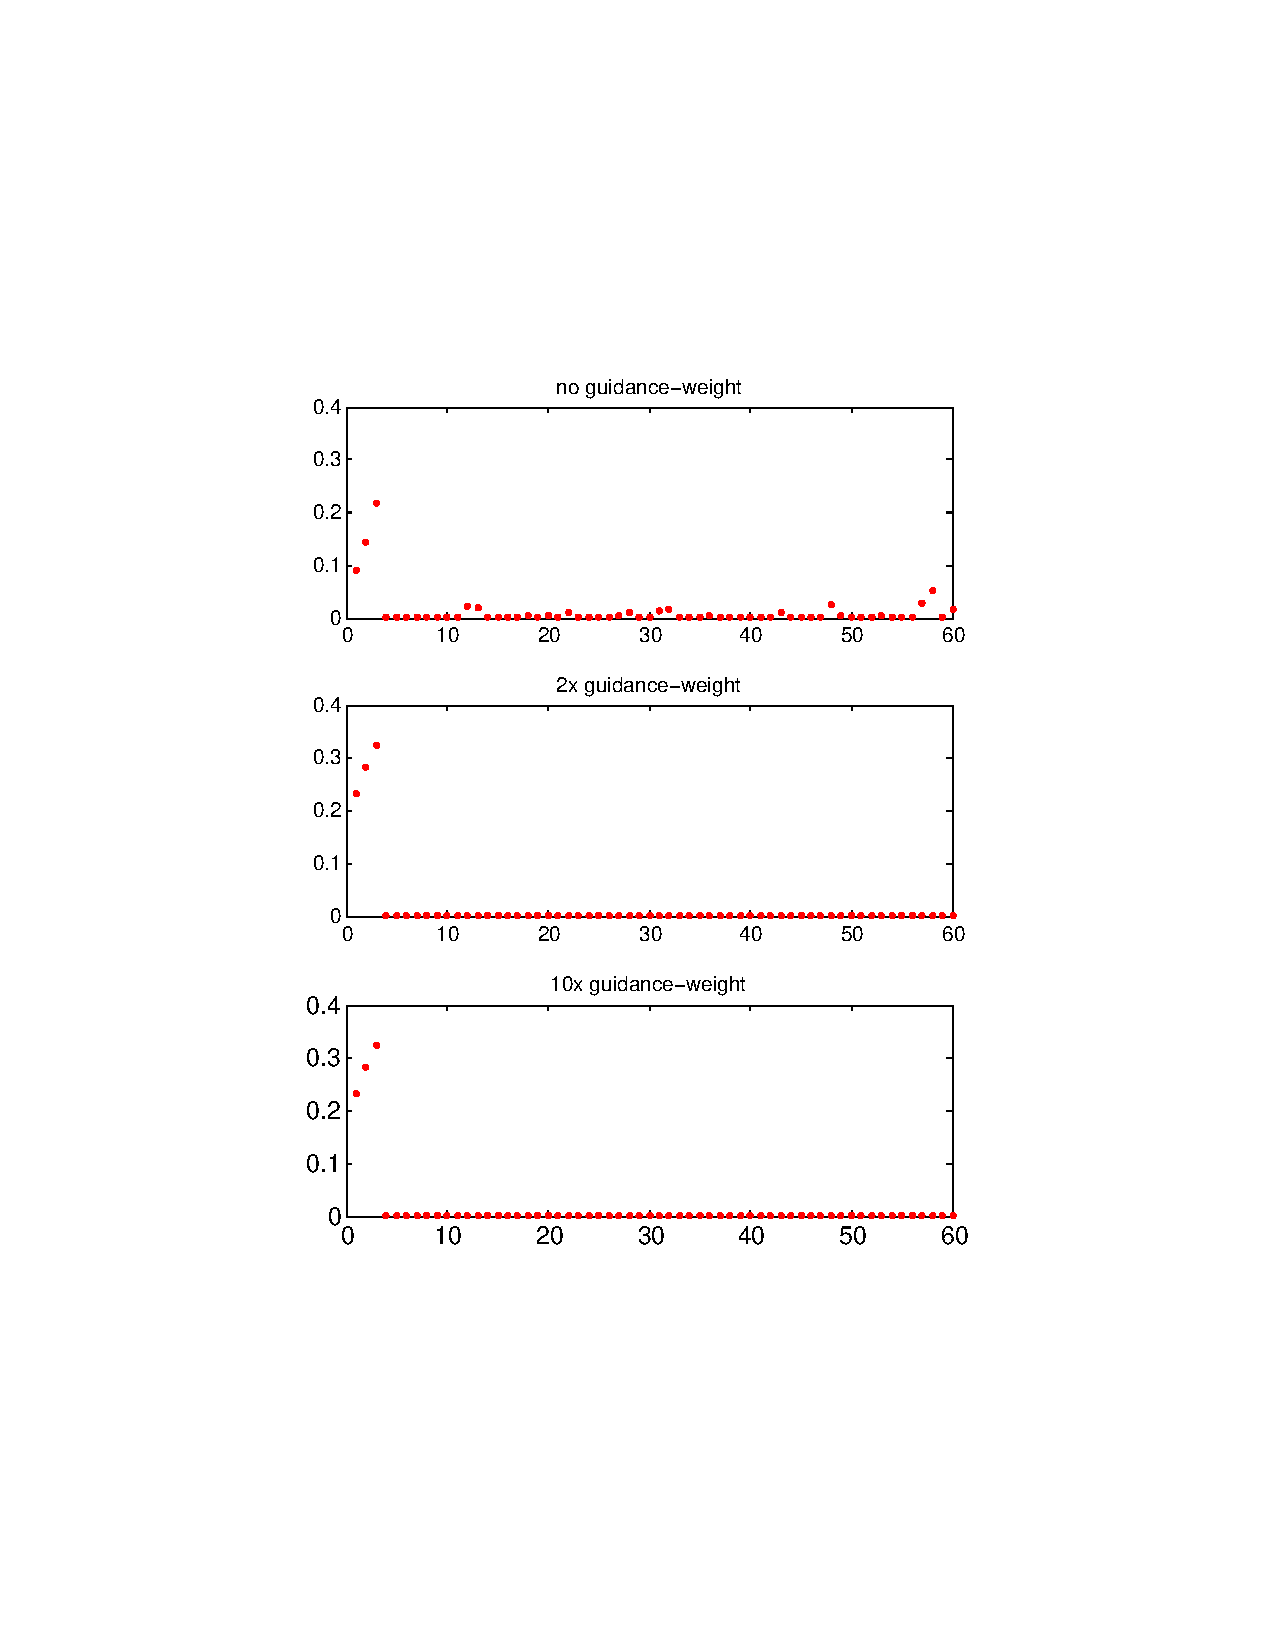
\includegraphics[trim= 150 200 150 200]{../code/figs/guided_recovery.pdf}
\end{figure}

\end{document}